\documentclass[a4paper,12pt]{book}
\usepackage[utf8]{inputenc}
\usepackage[spanish]{babel}
\usepackage{../common/sty/iramA4}
\usepackage{graphicx}
\usepackage{tikz}
\usepackage{fontawesome5}
\let\faPencil\faPen
\newcommand{\logo}{../common/img/4117.jpg}
\newcommand{\materia}{Mantenimiento}
\title{Guía de Trabajos Prácticos: \\
  Mantenimiento de Máquinas y Equipos \\
Agropecuarios}
\author{Escuela Técnica Agropecuaria}
\date{\today}

\begin{document}

\maketitle

\tableofcontents

\chapter{Introducción a la Gestión del Mantenimiento}
% Capítulo 1
\section*{Gestión Eficiente del Mantenimiento en el Ámbito Agropecuario}

\begin{center}
	\begin{tikzpicture}
		\node[inner sep=0pt, rounded corners=10pt] (myimage)
		{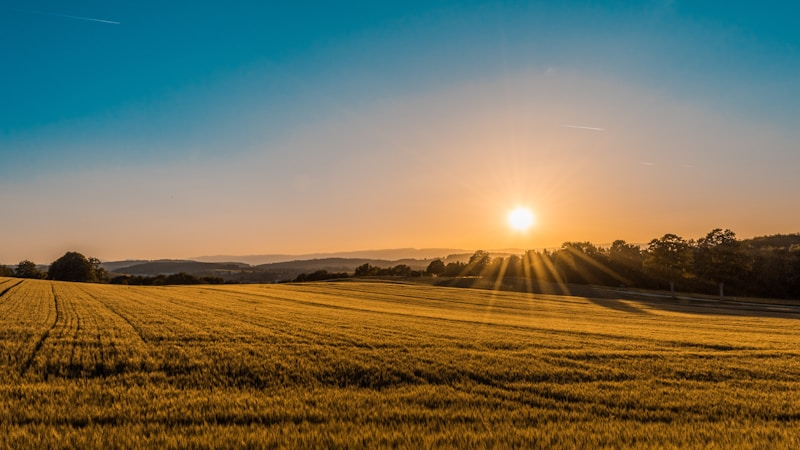
\includegraphics[width=0.6\textwidth,height=6cm]{img/cap1_mantenimiento.jpg}};
	\end{tikzpicture}
\end{center}

El mantenimiento agropecuario constituye la columna vertebral de la eficiencia
operativa en cualquier establecimiento productivo. En la actualidad, la
maquinaria agrícola representa una inversión de capital significativa, y su
disponibilidad operativa es crítica durante las ventanas de siembra o cosecha.

Una gestión inadecuada resulta no solo en reparaciones costosas, sino en
pérdidas productivas irreparables debido a tiempos de inactividad no
planificados. El objetivo del mantenimiento es maximizar la vida útil de los
equipos y asegurar que operen bajo condiciones óptimas de eficiencia.

\subsection*{Fundamentos del Mantenimiento}
El mantenimiento no se limita a reparar componentes averiados; es un proceso
estratégico de planificación. Se fundamenta en el conocimiento técnico, el
seguimiento de manuales del fabricante y la ejecución sistemática de tareas
orientadas a la confiabilidad.

\subsection*{Tipos de Mantenimiento}
\begin{itemize}
	\item \textbf{Mantenimiento Preventivo:} Realizado a intervalos predeterminados
	      según horas de uso o tiempo calendario. Busca prevenir fallas mediante
	      inspecciones, lubricación y reemplazo de componentes antes de su fallo.
	\item \textbf{Mantenimiento Correctivo:} Actuación reactiva tras la ocurrencia
	      de una falla. Es, por definición, el más costoso si afecta procesos
	      productivos críticos.
	\item \textbf{Mantenimiento Predictivo:} Basado en el monitoreo constante
	      de variables (temperatura, vibraciones, análisis de aceite) para
	      detectar indicios tempranos de degradación y predecir cuándo ocurrirá
	      una falla.
\end{itemize}

\subsection*{Herramientas Digitales para el Mantenimiento}
La digitalización en el sector agropecuario ha permitido el desarrollo de sistemas
de gestión de mantenimiento (CMMS) y herramientas de telemetría que permiten
un monitoreo en tiempo real del estado de los equipos. Estas herramientas facilitan
la planificación de servicios, el control de inventarios de repuestos y la reducción
de tiempos muertos mediante alertas automáticas basadas en horas de uso o sensores.

\section*{\faPencil\space Investigar y responder}
\begin{enumerate}
	\item ¿Cuál es la diferencia técnica entre el mantenimiento preventivo y el
	      correctivo en términos de costos operativos?
	\item Explique cómo el análisis de lubricantes (aceite) puede funcionar como una
	      técnica de mantenimiento predictivo.
	\item ¿Qué importancia tiene llevar un registro histórico (bitácora) de servicios
	      para un tractor con más de 2000 horas de uso?
	\item Defina el concepto de "disponibilidad mecánica" de una máquina agrícola.
	\item ¿Qué riesgos implica realizar mantenimiento correctivo como estrategia única
	      durante la temporada de cosecha?
	\item Investigue cuáles son las principales causas de degradación prematura en los
	      componentes de maquinaria agrícola bajo condiciones de campo (polvo,
	      humedad, carga).
	\item ¿Cómo impacta el mantenimiento preventivo en la seguridad del operador y del
	      personal del establecimiento?
	\item Defina qué se entiende por "ciclo de vida" de un activo agropecuario y cómo
	      la gestión de mantenimiento influye en él.
\end{enumerate}

\section*{\faWrench\space Resolver los siguientes problemas}
\begin{enumerate}
	\item Usted dispone de una cosechadora que requiere una inspección preventiva
	      cada 250 horas. La máquina lleva 1800 horas totales y su próximo servicio es
	      en 2000 horas. Calcule cuántos días operativos le quedan si el promedio de
	      uso diario es de 10 horas.
	\item Analice la siguiente situación: Un tractor pierde potencia repentinamente en
	      plena labor de siembra. Clasifique el tipo de mantenimiento que debe aplicar
	      y describa los pasos de diagnóstico iniciales.
	\item Elabore una tabla simple de chequeo diario (pre-uso) para un tractor,
	      incluyendo niveles de fluidos, presiones de neumáticos y estado de
	      iluminación.
	\item Compare dos lubricantes sintéticos y dos minerales de un catálogo técnico.
	      ¿Cuál recomendaría para condiciones de alta temperatura y por qué?
	\item Ante una falla recurrente en el sistema hidráulico, proponga una secuencia
	      de acciones de mantenimiento correctivo para evitar la recurrencia.
	\item Si un rodamiento falla a las 500 horas cuando el fabricante estima 1000,
	      ¿qué factores (uso, ambiente, lubricación) investigarían?
	\item Diseñe una tabla comparativa de costos proyectados (hipotéticos) para
	      realizar mantenimiento preventivo vs. correctivo en un tractor.
	\item Busque el manual de mantenimiento de un tractor de 100 HP e identifique los
	      intervalos de cambio de aceite y filtros de aire.
	\item Elabore un cronograma de mantenimiento preventivo mensual para una flota
	      compuesta por dos tractores y una cosechadora.
	\item Calcule la eficiencia de mantenimiento de una máquina que estuvo parada 20
	      horas de un total de 100 horas de disponibilidad programada.
\end{enumerate}


\chapter{Sistemas de Propulsión}
\section*{Sistemas de Propulsión y Motores de Combustión}

\begin{center}
	\begin{tikzpicture}
		\node[inner sep=0pt, rounded corners=10pt] (myimage)
		{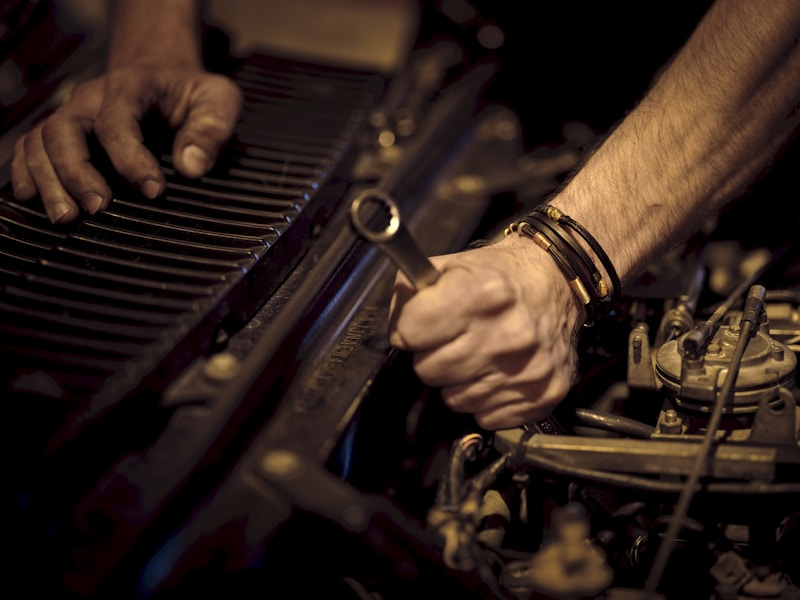
\includegraphics[width=0.6\textwidth,height=6cm]{img/cap2_motor.jpg}};
	\end{tikzpicture}
\end{center}

El motor de combustión interna, particularmente el motor Diesel, representa el corazón
energético de la maquinaria agrícola. Su función principal es transformar la energía
química contenida en el combustible en energía mecánica utilizable para tracción y
accionamiento de implementos. Comprender su funcionamiento es fundamental para un
mantenimiento que garantice potencia, eficiencia y una larga vida útil.

\subsection*{Fundamentos del Ciclo Diesel}
A diferencia de los motores de encendido por chispa, el motor Diesel utiliza el
calor generado por la alta compresión del aire en la cámara de combustión para
ignorar el combustible inyectado. Este ciclo, compuesto por las fases de admisión,
compresión, combustión/expansión y escape, requiere un control preciso de la
mezcla aire-combustible y de la temperatura operativa para maximizar el rendimiento.

\subsection*{Sistemas Auxiliares}
Para garantizar una operación eficiente, el motor depende de sistemas críticos:
\begin{itemize}
	\item \textbf{Sistema de Lubricación:} Reduce la fricción y disipa el calor en
	      partes móviles (pistones, cigüeñal, árbol de levas).
	\item \textbf{Sistema de Refrigeración:} Mantiene la temperatura dentro de los
	      rangos óptimos de trabajo, evitando deformaciones por dilatación térmica.
	\item \textbf{Sistema de Alimentación y Filtrado:} Asegura el suministro de
	      combustible y aire limpios, vital para prevenir el desgaste prematuro de
	      bombas e inyectores.
\end{itemize}

\section*{\faPencil\space Investigar y responder}
\begin{enumerate}
	\item Explique detalladamente la diferencia técnica entre el ciclo de trabajo de
	      un motor Diesel y un motor naftero (Otto).
	\item ¿Cuál es la función específica del termostato en el sistema de
	      refrigeración y qué consecuencias implica su mal funcionamiento?
	\item Describa la importancia de la viscosidad del aceite lubricante y cómo
	      afecta el desempeño del motor en climas extremos.
	\item ¿Qué papel juega el turbocompresor en el aumento de potencia de los motores
	      agrícolas modernos?
	\item ¿Qué indica la presencia de humo negro, azul o blanco por el escape de un
	      tractor Diesel?
	\item Explique qué es la relación de compresión y por qué es superior en los
	      motores Diesel.
	\item ¿Cuál es la función del sistema de filtrado de combustible y por qué el
	      agua es un contaminante crítico?
	\item Investigue los efectos de la sobrecarga operativa en la vida útil de los
	      componentes del tren alternativo del motor.
\end{enumerate}

\section*{\faWrench\space Resolver los siguientes problemas}
\begin{enumerate}
	\item Dado un manual de mantenimiento, identifique el intervalo de cambio de
	      aceite y filtros para un motor de 150 HP y justifique si debe acortarse en
	      condiciones de alta polución.
	\item Un tractor presenta dificultades de arranque en frío. Proponga una
	      secuencia de diagnóstico para el sistema de alimentación y precalentamiento.
	\item Calcule el volumen de refrigerante necesario para un sistema cuya capacidad
	      total es de 20 litros, considerando una mezcla recomendada de 50/50.
	\item Analice el desgaste prematuro de un conjunto camisa-pistón. ¿Qué pruebas
	      realizaría para determinar si la causa es lubricación deficiente o
	      filtración de aire?
	\item Diseñe una hoja de registro para el seguimiento del consumo de aceite
	      lubricante entre servicios, incluyendo el horómetro de la máquina.
	\item Ante una pérdida de potencia notable, ¿cómo realizaría una prueba de
	      estanqueidad de cilindros?
	\item Describa el procedimiento paso a paso para purgar aire del sistema de
	      combustible en un motor Diesel tras un cambio de filtros.
	\item Si la temperatura de operación supera los 100°C, enumere los componentes
	      críticos a inspeccionar (radiador, bomba, sensores).
	\item Calcule el consumo horario de combustible de un tractor que operó 8 horas y
	      requirió 120 litros para rellenar el tanque al máximo.
	\item Investigue y explique el proceso de regulación de luz de válvulas en un
	      motor agrícola convencional.
\end{enumerate}


\chapter{Transmisiones y Sistemas de Potencia}
\section*{Transmisiones y Sistemas de Potencia}

\begin{center}
	\begin{tikzpicture}
		\node[inner sep=0pt, rounded corners=10pt] (myimage)
		{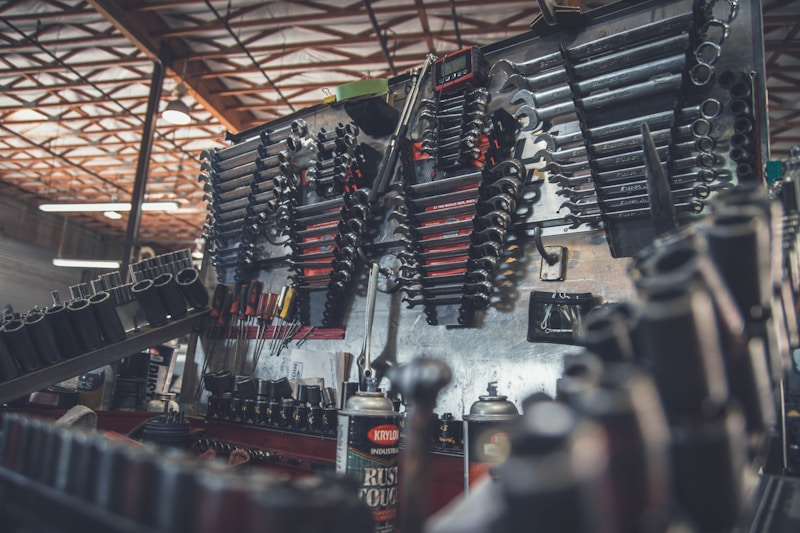
\includegraphics[width=0.6\textwidth,height=6cm]{img/cap3_transmision.jpg}};
	\end{tikzpicture}
\end{center}

El sistema de transmisión es el encargado de canalizar la potencia generada por el
motor hacia las ruedas motrices y la Toma de Fuerza (TDF), permitiendo que el tractor
desarrolle la fuerza de tracción necesaria para las labores agrícolas. Un sistema
robusto y bien mantenido es crucial para operar eficientemente bajo diversas cargas
y terrenos.

\subsection*{Fundamentos de la Transmisión}
La transmisión transforma el alto régimen de giro y bajo torque del motor en una
salida de bajo régimen y alto torque en las ruedas. Este proceso involucra una
serie de engranajes, embragues y ejes que deben trabajar bajo condiciones de alta
presión y temperatura.

\subsection*{Componentes del Sistema}
\begin{itemize}
	\item \textbf{Embrague:} Conecta y desconecta el motor de la transmisión.
	\item \textbf{Caja de Cambios:} Proporciona las diferentes relaciones de
	      velocidad y sentido de marcha.
	\item \textbf{Diferencial y Mandos Finales:} Distribuyen la potencia a las ruedas,
	      permitiendo velocidades distintas en curvas.
	\item \textbf{Toma de Fuerza (TDF):} Transmite potencia mecánica directa a
	      implementos como desmalezadoras o pulverizadoras.
\end{itemize}

\section*{\faPencil\space Investigar y responder}
\begin{enumerate}
	\item Describa la diferencia operativa entre un embrague mecánico y uno de discos
	      múltiples bañados en aceite.
	\item ¿Cuál es la función del diferencial en un tractor y por qué es crítico su
	      ajuste en labores de alta tracción?
	\item Investigue los tipos de cajas de cambios agrícolas: manuales, sincronizadas
	      y Powershift (o IVT). Ventajas y desventajas.
	\item Explique la importancia de la Toma de Fuerza (TDF) y las precauciones de
	      seguridad asociadas a su uso.
	\item ¿Por qué es fundamental utilizar lubricantes específicos (tipo UTTO o
	      STOU) para transmisiones que comparten aceite con sistemas hidráulicos?
	\item ¿Qué función cumplen las crucetas y los ejes cardánicos en la transmisión
	      de potencia a implementos remolcados?
	\item Investigue las causas principales de desgaste prematuro en los engranajes
	      de la caja de velocidades.
	\item ¿Qué diferencia el funcionamiento de un sistema de tracción 4x2 respecto a
	      un 4x4 bajo condiciones de terreno blando?
\end{enumerate}

\section*{\faWrench\space Resolver los siguientes problemas}
\begin{enumerate}
	\item Ante un ruido metálico al cambiar de marcha, proponga una secuencia de
	      diagnóstico para identificar el componente fallido.
	\item Calcule el volumen de aceite necesario para una transmisión cuya capacidad
	      total es de 45 litros, si se han drenado solo 38 litros.
	\item Diseñe una tabla de inspección de los ejes cardánicos, incluyendo puntos de
	      engrase y estado de los protectores de seguridad.
	\item Un tractor pierde tracción en una rueda trasera. ¿Qué componentes del
	      diferencial y mandos finales inspeccionaría primero?
	\item Elabore un procedimiento para el ajuste de la carrera libre del pedal de
	      embrague.
	\item Analice el sobrecalentamiento en la carcasa de la caja de cambios tras una
	      jornada de labranza pesada. ¿Qué variables (carga, lubricante) revisar?
	\item Si la TDF no se desacopla, ¿qué fallas mecánicas podría investigar en el
	      mecanismo de accionamiento?
	\item Compare la eficiencia teórica de transmisión de potencia entre un sistema
	      mecánico directo y uno hidrostático.
	\item Elabore un cronograma de lubricación para los ejes delanteros de un tractor
	      4x4 según horas de uso.
	\item Ante una fuga de lubricante por el retén del eje de la TDF, describa el
	      procedimiento de reemplazo y las precauciones necesarias.
\end{enumerate}


\chapter{Sistemas Hidráulicos}
\section*{Sistemas Hidráulicos en Equipos Agrícolas}

\begin{center}
	\begin{tikzpicture}
		\node[inner sep=0pt, rounded corners=10pt] (myimage)
		{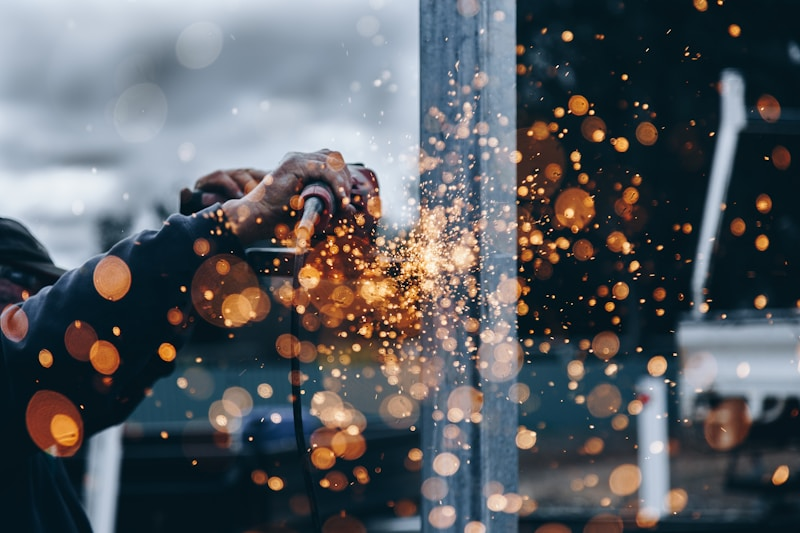
\includegraphics[width=0.6\textwidth,height=6cm]{img/cap4_hidraulica.jpg}};
	\end{tikzpicture}
\end{center}

El sistema hidráulico en la maquinaria agrícola moderna actúa como el sistema
muscular, permitiendo el control preciso y la transmisión de fuerza necesaria
para operar implementos (arados, sembradoras, palas cargadoras) con alta eficiencia.
La correcta gestión de estos sistemas es crítica para evitar fallas catastróficas
debido a las altas presiones operativas.

\subsection*{Fundamentos del Sistema}
El funcionamiento se basa en el Principio de Pascal: la presión aplicada a un fluido
contenido en un recipiente cerrado se transmite con la misma intensidad en todas las
direcciones. Este principio permite multiplicar fuerzas a partir de un flujo de
aceite a presión generado por una bomba mecánica.

\subsection*{Componentes Clave}
\begin{itemize}
	\item \textbf{Bomba Hidráulica:} Genera el flujo necesario para el sistema.
	\item \textbf{Válvulas de Control:} Regulan la dirección, presión y caudal del
	      fluido hacia los actuadores.
	\item \textbf{Actuadores (Cilindros/Motores):} Convierten la energía hidráulica
	      en movimiento mecánico lineal o rotativo.
	\item \textbf{Depósito y Filtrado:} Almacenan y aseguran la limpieza del fluido.
\end{itemize}

\section*{\faPencil\space Investigar y responder}
\begin{enumerate}
	\item Explique el Principio de Pascal y cómo se aplica para levantar un implemento
	      pesado con un cilindro pequeño.
	\item ¿Qué diferencia técnica existe entre una bomba hidráulica de engranajes y
	      una de pistones de caudal variable?
	\item ¿Cuál es la función de la válvula de alivio (de seguridad) y por qué es
	      peligroso anularla?
	\item Defina qué es la "cavitación" en una bomba hidráulica y cómo afecta su
	      vida útil.
	\item ¿Por qué la presencia de aire en el sistema hidráulico genera ruidos y
	      movimientos erráticos?
	\item Investigue los efectos de la contaminación (partículas sólidas y agua) en
	      el desgaste de las válvulas de control.
	\item ¿Qué medidas de seguridad extrema deben tomarse al inspeccionar mangueras
	      hidráulicas bajo presión (riesgo de inyección de fluido)?
	\item Describa la importancia de los filtros hidráulicos y la diferencia entre
	      filtros de succión y de retorno.
\end{enumerate}

\section*{\faWrench\space Resolver los siguientes problemas}
\begin{enumerate}
	\item Utilizando un manómetro, describa el procedimiento para verificar la
	      presión de trabajo máxima de un circuito de control remoto.
	\item Proponga un método para detectar fugas internas en un cilindro hidráulico
	      sin desmontarlo de la máquina.
	\item Si el fluido hidráulico presenta un color lechoso, ¿qué indica y qué
	      acciones correctivas deben seguirse?
	\item Calcule la fuerza de elevación de un cilindro con un émbolo de 10 cm de
	      diámetro trabajando a una presión de 150 bar.
	\item Elabore un protocolo de limpieza antes de desconectar acoples rápidos para
	      evitar la entrada de polvo al sistema.
	\item Analice el sobrecalentamiento constante del aceite hidráulico. ¿Qué
	      componentes del sistema (enfriador, válvulas) inspeccionaría?
	\item Describa el procedimiento paso a paso para reemplazar los sellos (o'rings)
	      de un cilindro que presenta fugas externas.
	\item Calcule el volumen necesario de aceite para un sistema que requiere
	      llenado total, sabiendo que el depósito tiene 40 litros y los circuitos
	      adicionales contienen 15 litros.
	\item Diseñe una tabla de mantenimiento para el cambio de filtros y análisis de
	      calidad de aceite según horas de uso.
	\item Ante una respuesta lenta del sistema hidráulico, enumere las causas
	      probables (bomba, niveles, viscosidad) y cómo descartarlas.
\end{enumerate}


\chapter{Seguridad Industrial y Herramientas}
\section*{Seguridad Industrial y Taller}

\begin{center}
	\begin{tikzpicture}
		\node[inner sep=0pt, rounded corners=10pt] (myimage)
		{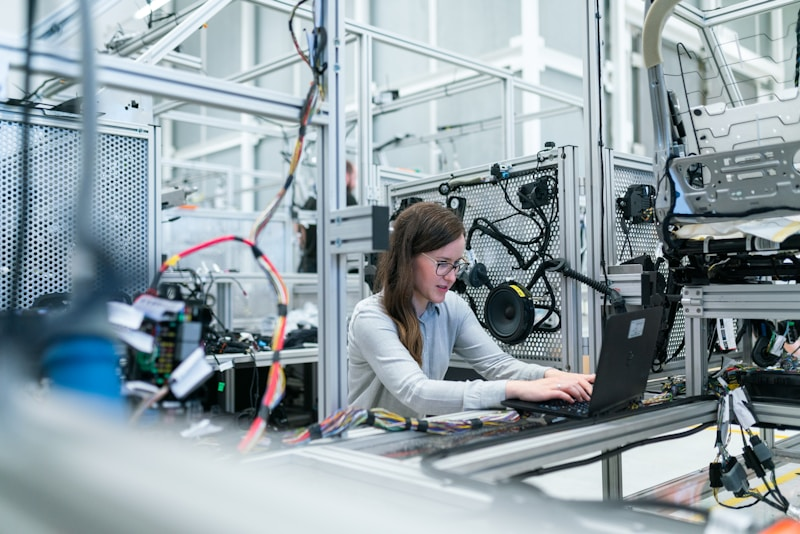
\includegraphics[width=0.6\textwidth,height=6cm]{img/cap5_seguridad.jpg}};
	\end{tikzpicture}
\end{center}

El mantenimiento seguro constituye un pilar fundamental en cualquier establecimiento
agropecuario. La prevención de accidentes no solo protege la integridad física de
los operadores y personal técnico, sino que también garantiza la continuidad
operativa evitando paralizaciones por incidentes laborales.

\subsection*{Fundamentos de la Prevención}
La seguridad industrial se basa en la identificación y mitigación de riesgos.
Implica establecer procedimientos de trabajo seguros (PTS), mantener el orden y la
limpieza (metodología 5S), y garantizar el uso correcto de equipamiento.

\subsection*{Equipamiento de Protección Personal (EPP)}
El EPP es la última barrera de defensa. Todo personal debe contar con:
\begin{itemize}
	\item \textbf{Protección Craneal y Facial:} Cascos y protectores auditivos/oculares.
	\item \textbf{Protección Respiratoria:} Mascarillas ante polvo o químicos.
	\item \textbf{Protección dérmica:} Guantes, calzado de seguridad y ropa adecuada.
\end{itemize}

\section*{\faPencil\space Investigar y responder}
\begin{enumerate}
	\item Enumere las normas básicas de seguridad para el trabajo en el taller agrícola.
	\item ¿Qué EPP es obligatorio para tareas de soldadura y por qué?
	\item Investigue los tipos de extintores (clases A, B, C) y cuál es el adecuado
	      para un incendio de combustible.
	\item ¿Cuáles son las medidas preventivas fundamentales para el almacenamiento
	      seguro de combustibles (gasoil) y lubricantes?
	\item Explique los riesgos inherentes de trabajar sobre maquinaria en marcha o con
	      sistemas hidráulicos bajo presión.
	\item ¿Qué es un torquímetro y cuál es su importancia para evitar la rotura de
	      tornillos críticos?
	\item Describa brevemente los principales tipos de soldadura utilizados en campo
	      y sus riesgos asociados.
	\item ¿Por qué el orden y la limpieza son considerados pilares de la seguridad en
	      el taller?
	\item Identifique los riesgos eléctricos al utilizar herramientas portátiles en
	      ambientes húmedos o metálicos.
	\item Diseñe un procedimiento básico de emergencia ante un accidente laboral en
	      el campo (puntos a comunicar, botiquín).
\end{enumerate}

\section*{\faWrench\space Resolver los siguientes problemas}
\begin{enumerate}
	\item Realice una inspección visual de un equipo de protección y elabore una
	      lista de chequeo para determinar si está apto para su uso.
	\item Diseñe un plan de evacuación y emergencia para su área de trabajo,
	      identificando salidas y puntos de reunión.
	\item Seleccione las herramientas manuales adecuadas para una tarea específica y
	      justifique su elección basándose en la seguridad.
	\item Practique el uso correcto de un torquímetro para apretar un tornillo de
	      bancada según las especificaciones del manual.
	\item Organice su área de trabajo aplicando la metodología 5S y documente el
	      "antes" y el "después".
	\item Identifique tres situaciones de riesgo potencial en su taller y proponga
	      acciones correctivas inmediatas.
	\item Diseñe un mapa de señalización de seguridad para el taller (salidas,
	      extintores, zonas de alta tensión).
	\item Clasifique los residuos peligrosos generados en el mantenimiento (aceites
	      quemados, filtros, baterías) y defina su disposición final.
	\item Realice una inspección técnica de herramientas manuales (martillos, llaves)
	      buscando desgastes o fisuras peligrosas.
	\item Planifique y ejecute un simulacro de emergencia ante un derrame de
	      combustible o incendio menor.
\end{enumerate}


\end{document}
